\documentclass[letter,openright,12pt,spanish]{report}

\title{\textbf{Describir los métodos geométricos algebraicos y desacoplo cinemático.}}
\title{\begin{center}

\includegraphics[scale=1.5]{Escudo.png} 
\end{center}Describir los métodos geométricos algebraicos y desacoplo cinemático}
\author{Fonseca Camarena Jonathan.\\
		Ing. Mecatr\'onica}
\date{22 de octubre de 2019}
\usepackage{amsmath}
\usepackage{graphicx}
\begin{document}




\maketitle

\section{Cinem\'atica Directa}

El problema cinem\'atico directo consiste en determinar cu\'al es la posici\'on y orientaci\'on del extremo final del robot, con respecto a un sistema de coordenadas que se toma como refrencia, conocidos los valores de las posiciones articulares y los par\'ametros geom\'tricos de los elementos del robot. 

\begin{displaymath}
x=\textit{f}(q)
\end{displaymath}

En general, un robot de "n" grados de libertad est\'a formado por "n" eslabones unidos por "n" articulaciones, de forma que cada par articulaci\'on-eslab\'on constituyen un grado de libertad. A cada eslab\'on se le puede asociar un sistema de refrencia solidario a \'el y, utilizando las transofmaciones homog\'eneas, es posible representar las rotaciones y traslaciones relativas entre los distintos eslabones que componen el rbot. La matriz de transformaci\'on homog\'enea que representa la posici\'on y orientaci\'on relativa entre los distintos sistemas asociados a dos eslabones consecutivos del robot se denomina $^{i-1}A_i$. Del mismo modos, la matriz $^0A_k$, resultante del producto de las matrices $^{i-1}A_i$ con i desde 1 hasta k, es la que representa de forma total o parcial la cadena cinem\'atica que forma el robot con respecto al sistema de referencia inercial asociado a la base. Cuando se considera todos los grados de libertad, a la matriz $^0A_n$ se le denomina T, matriz de transformaci\'on que relaciona la posici\'on y orientaci\'on del extremo final del robot respecto del sistema fijo situado en la base del mismo. As\'i, dado un robot de 6 gdl, se tiene que la osici\'on y orientaci\'on del eslab\\on final vendr\'a dado por la matriz T:\\

\begin{displaymath}
T=^0A_1 \cdot ^1A_2 \cdot ^2A_3... ... ^nA_n
\end{displaymath} 

Para describir la relaci\'on que existe entre dos sistemas de referencia asociados a eslabones, se utiliza la representaci\'on Denavit-Hartenberg (D-H). 

\section{Cinematica Inversa}

EL problema cinem\'atico inverso consiste en encontrar los valores que deben adoptar las coordenadas articulares del robot [ $\textit{q=q}_1,\textit{q}_2,...,\textit{q}_n$ ] para que su extremo se posicione y oriente seg\'un una determinada localizaci\'on espacial. Al contrario que el problema cinem\'atico directo, el c\'alculo de la cinam\'atica inversa no es sencilla ya que conssite en la resoluci\'on de una serie de ecuaciones fuertemen dependiente de la configuraci\'on del robot, adem\'as de existir diferentes \textit{n-uplas} [$\textit{q=q}_1,\textit{q}_2,...,\textit{q}_n$ ] que resuelve el problema.
En la actualidad existen procedimientos gen\'ericos susceptibles de ser progrmados para la resoluci\'on de la cinem\'atica inversa y obtener la \textit{n-upla} de valores articulares que posionen y orienten el extremo final. Sin embargo, el principla inconveniente de estos procedimientos es que son m\'etodos num\'ericos iterativos, que no siempre garantizan tener la soluci\'on en el momento adecuado. De esta manera, a la hora de resolver el problema cinem\'atico inverso es mucho m\'as adecuado encontrar una soluci\'on cerrada. Es decir, encontrar una relaci\'on matem\'atica expl\'icita de la forma:

\begin{displaymath}
q_k=f_k(x, y, z, \alpha, \beta, \gamma)
\end{displaymath}

\begin{displaymath}
k=1...n (grados de libertad)
\end{displaymath}

Para poder conseguir esta relaci\'on suele ser habitual emplear geom\'etricos, que consisten en la utilizaci\'on de las relaciones trigonom\'etricas y la resoluci\'on de los tr\'iangulos formados por los elementos y articulaciones del robot. La mayor\'ia de los robots suele tener cadenas cinem\'aticas relativamente sencillas, y los tres primeros grados de libertad (gdl), que posicionan al robot en el espacio, suelen tener una estructura planar. Esta condici\'on facilita la resoluci\'on de la \textit{n-upla}. Adem\'as, los tres \'ultimos grados de libertad suelen usarse para la orientaci\'on de la herramienta, lo cual permite la resoluci\'on desacolada (descoplo cinem\'atico) de la posici\'on del extremo del robot y de la orientaci\'on de la herramienta. Como alternativa para reoslver el mismo problema se puede recurrir a manipular directamente las ecuaiciones correspondientes al problema cinem\'atico directo. Es decir, a partir de la relaci\'on entre la matriz de transformaci\'on y las ecuaciones en funci\'on de las coordenadas articulares $\textit{q=[q}_1,\textit{q}_2,\textit{q}_3,...,\textit{q}_n]$, es posible despejar las n variables articualaciones $q_i$ en funci\'on de las componentes de los vectores \textbf{n}, \textbf{o}, \textbf{a} y \textbf{p}:

\begin{center}
[
$\begin{matrix}
	n & o & a & p\\
	0 & 0 & 0 & 1\\
\end{matrix}$ ] = [$t_ij$($q_i$,...$q_n$)]
\end{center}

Donde los elementos $t_{ij}$ son funciones de las coordenadas articulares ($q_i$,...,$q_n$)$\cdot $ $e^t$.

La matriz de tranfomaci\'on homog\'enea es una matriz 4 x 4 que transforma un vector de posici\'on expresado en coordenadas homog\'enas desde un sistema de coordenado a otro. En general se representa:

\begin{center}
T = [ $\begin{matrix}
	R_{3x3} & P_{3x1}\\
	F_{1x3} & 1x1\\
\end{matrix}$ ] = [$\begin{matrix}
	\textbf{rotaci\'on} & \textbf{traslaci\'on}\\
	\textbf{perspectiva} & \textbf{escaldo}\\
\end{matrix}$
\end{center}

\section{Metodo Geom\'etrico}

El m\'etodo gemoetrico explota la configuraci\'on de un manipulador particular para resolver por medio de relaciones geom\'etricas planas los valores de cada \'angulo de articulaci\'on. A continuaci\'on se presenta una soluci\'on geom\'etrica para el robot Mitsubushi RV-M1.

\begin{figure}[htp]
\centering
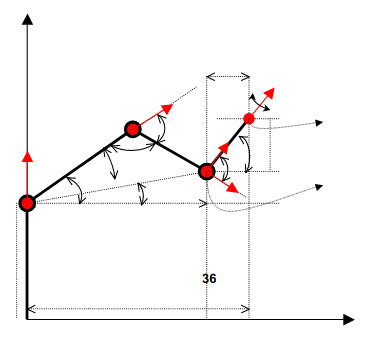
\includegraphics[width=8cm]{1.jpg}
\caption{RV-M1}
\label{Figura 1}
\end{figure}

La soluci\'on para la articulaci\'on de cintura est\'a dad por:

\begin{displaymath}
\theta_1=atan2(p_y,p_x)
\end{displaymath}

Es posible, dada la configuraci\'on cinem\'atica del Mitsubishi RV-M1, simplifacar el conjunto de par\'ametros requeridos para solucionar las variables siguientes (eliminando las coordenadas sobre el eje "y") llevando la geometr\'ia a coincidencia con un solo plano, tal y como se muestra en la la figura anterior (plano xz). Para ellos es necesario aplicar una rotaci\'on de $-\theta_1$ alrededor del eje $z_0$ sobre la matriz de transofrmaci\'on homog\'enea que expresa la posici\'on y orientaci\'on del efector final El resultado se utilizar\'ia eentonces para hallar las variables del \'angulo siguientes.

\begin{displaymath}
Tn^0_5=T_{z_{0}-\theta_1}T^0_5
\end{displaymath}

Sin embargo, tomaremos la v\'ia convencional.

En primera instancia determinamos el punto coincidente con el origen de la articulaci\'on de mu\~neca.

\begin{displaymath}
p_m=p-d_3a
\end{displaymath}

Donde, $\alpha $ corresponde al vector unitario de aproximaci\'on del efecto extra\'ido de $T^0_5$, $d_5$ al largo del efecto final y \textit{p} al subvector de posici\'on extra\'ido de $T^0_5$.

La distancia entre el eje de articulaci\'on del hombro y el eje de la mu\~neca ($\textit{p}_m$) est\'a dado por,

\begin{displaymath}
R=\sqrt{p^2_m+p^2_m+(p^2_{m_x}-d_1)^2}
\end{displaymath}

Encontrando el  \'angulo parcial asociado con el hombro,

\begin{displaymath}
\theta_{2a}=atan2(p_m,\sqrt{p^2_{m_x}+p^2_{m_y}})
\end{displaymath}

y aplicando la ley de cosenos para resolver por $0\leq \theta_{2b}\leq \pi$ de tal manera que se preserva la geometr\'ia

\begin{displaymath}
\theta_{2b}=|acos(\frac{R^2+a^2_2-a^2_3}{2a_2R})|
\end{displaymath}

Entonces,

\begin{center}
$\theta_2$=\{ $\begin{matrix}
	\theta_{2b} & -\theta_{2a} & si R \leq (a_2+a_3)\\
	\theta_{2a} & -\theta_{2b} & si R \succ (a_2+a_3)\\
\end{matrix}$
\end{center}

$z_0$ Nuevamente empleando la ley de cosenos para halar la variable de articulaci\'on n \'umero tres ($\theta_3$)

\begin{displaymath}
\theta_3=-|acos(\frac{R^2-a^2_2-a^2_3}{2a_2a_3})|
\end{displaymath}

El signo de $\theta_3$ es simepre negativo, debido a la limitaci\'on en movimiento del codo en este manipulador.

Estos tres primeros \'angulos de arituclaci\'on representan la posici\'on de la mu\~neca en el espacio eucl\'ideo tridimencional. Empleando estos resultados parciales para encontrar la posici\'on y orientaci\'on de la mu\~neca podemos deducir rapidamente los \'angulos restantes que otorgan la orientaci\'on de la misma.

\begin{displaymath}
T^0_3=A^0_1(\theta_1)A^1_2(\theta_2)A^2_3(\theta_3)
\end{displaymath} 

El vector de aproximaci\'on de la mano, $\alpha $, se extrae directamente de $T^0_5$ y seg\'un la morfolog\'ia del manipulador se orienta en el sentido del elemento $d_5$ y es referenciado con respecto del sistema de base del robot. Examinando la geometr\'ia del efecto final, de manera m\'as precisa la orientaci\'on de los vectores de la mano estra\'idos de $T^0_5$, en relaci\'on con $T^0_3$ encontramos que el movimiento de "pitch" est\'a siempre sobre el plano de $\theta_1$.

\begin{figure}[htp]
\centering
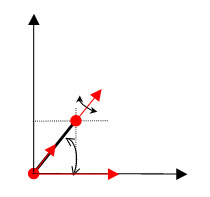
\includegraphics[width=8cm]{3.jpg}
\caption{Esquematico 2}
\label{Figura 2}
\end{figure}

Consecuentemene,

\begin{displaymath}
sen(\theta_4)=a'\cdot w_3
\end{displaymath}

\begin{displaymath}
cos(\theta_4)=a'\cdot u_3
\end{displaymath}

\begin{displaymath}
\theta_4=atan2(a^T\cdot u_3,a^T\cdot w_3)
\end{displaymath}

De igual manera para $\theta_5$, encontramos $T^0_4$, y evaluamos las proyecciones de $T^0_5$, sobre el sistema de coordenadas resultante,

\begin{displaymath}
sen(\theta_5)=n^T\cdot v_4
\end{displaymath}

\begin{displaymath}
cos(\theta_5)=o^T \cdot v_4
\end{displaymath}

\begin{displaymath}
\theta_5=atan2(n^T\cdot v_4, o^T \cdot v_4)
\end{displaymath}

Es de notar que para el caso del \'angulo de "roll" se utiliza el vector de deslizamiento/orientaci\'on de la u\~na.

\textbf{Caracteristicas del Metodo Geom\'etrico}

Es un m\'etodo no sistem\'atico que \'utiliza las relaciones geom\'etricas para obtener la posici\'on del extremo del robot.

Normalmente se emplea para la obtenci\'on de la posici\'on y no de la orientaci\'on.

Se usan en robots de pocos grados de libertad.

\begin{figure}[htp]
\centering
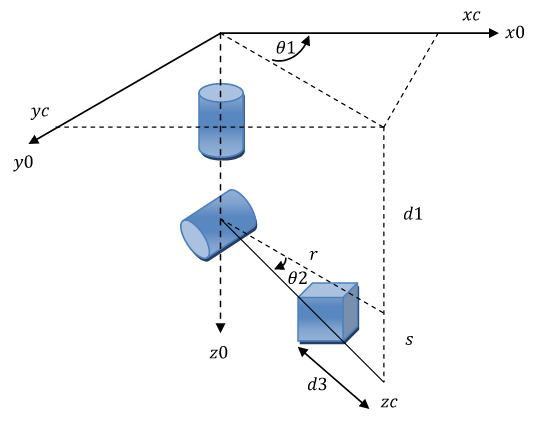
\includegraphics[width=8cm]{2.jpg}
\caption{Caracteiristicas del metodo geom\'etrico}
\label{Figura 3}
\end{figure}

\section{Metodo Algebraico}

Como se discut\'io en la secci\'on anterior s\'olo en casos especiales pueden los robots manipuladores resolverse de manera cerrada y anal\'itica. Para ello el manipulador debe cumplir alguna de las siguientes condiciones:

Tres ejes de articulaci\'on adyacentes intersectantes en un punto y/o muchos $\alpha_i$ iguales a 0 $\pm$ 90 grados.

Tres ejes de articulaci\'on adyacentes son paralelos entre s\'i (condici\'on suficiente).

Las siguientes equivalentes trigonometricas son de gran utilidad para simplificar las expreciones matriciales a partir de las condiciones anteriore:

\begin{displaymath}
sen(a+b)=sen(a)cos(b)+cos(a)sen(b)
\end{displaymath}

\begin{displaymath}
cos(a+b)=cos(a)cos(b)-sen(a)sen(b)
\end{displaymath}

\begin{displaymath}
sen(a+b+c)=sen(a)cos(b)cos(c)+cos(a)sen(b)cos(c)-sen(a)sen(b)sen(c)+cos(a)cos(b)sen(c)
\end{displaymath}

\begin{displaymath}
cos(a+b+c)=cos(a)cos(b)cos(c)-sen(a)sen(b)cos(c)-sen(a)cos(b)sen(c)-cos(a)sen(b)sen(c)
\end{displaymath}

El siguiente m\'etodo se le atribuye a Paul y consiste en encontrar cada variable de manera secuencial, aisalado cada una mediante la premultiplicaci\'on las correspondientes transformadas inversas, como se indica en las ecuaciones (\textsc{aqu\'i quedamos}). Para el caso de un manipulador de 6 grados de libertad los productos de las transformaciones dadas en las matrices homog\'enea 4x4, comenzando desde la articulaci\'on 6 hasta llegar a la base del robot est\'an dados por; seis ecuaiones matriales se pueden obtener a partir de esta ecuaci\'on, pre-multiplicandola sucesivamente por las inversas de las matrices A.

\begin{displaymath}
(A^0_1)^{-1}T^0_6=T^1_0
\end{displaymath}

\begin{displaymath}
(A^1_2){-1}(A^0_1)^{-1}T^0_6=T^2_6
\end{displaymath}

\begin{displaymath}
(A^2_3)^{-1}(A^1_2)^{-1}(A^0_1)^{-1}T^0_6=T^3_6
\end{displaymath}

\begin{displaymath}
(A^3_4)^{-1}(A^2_3)^{-1}(A^1_2)^{-1}(A^0_1)^{-1}T^0_6=T^4_6
\end{displaymath}

\begin{displaymath}
(A^4_5)^{-1}(A^3_4)^{-1}(A^2_3)^{-1}(A^1_2)^{-1}(A^0_1)^{-1}T^0_6=T^5_6
\end{displaymath}

El procedimineto consiste en revisar los elementos del lado derecho de las ecuaciones, encontrar aquellos que sean cero o constantes, e igualarlos con los elementos respectivos del lado izquierdo de la ecuaci\'on.

La matriz homog\'enea $T^0$ qie especifican la localizaci\'on del sistema de coordenadas i-\'esimo con respecto al sistema de coordenadas de la base esta dado por;

\begin{center}
$T^0_i=A^0_1A^1_2...A^{i-1}_i= \prod^i_{j=1}A_j^{j-1}$ =[$\begin{matrix}
	R^0_j & p^0_i\\
	0 & 1\\
\end{matrix}$]
\end{center}

$i=1,2,...,n$\\

Donde;\\

$\textbf{R}^0_i$:  Matriz de orientaci\'on del sistema de coordenadas i-\'esimo establecido en el elemento i con respecto al sistema de coordenadas de la base. Es la submatriz superior izquierda de 3x3 de $T^0_i$

$\textbf{p}^0_1$: Vector de posici\'on que apunta desde el origen del sistema de coordenadas de la base hasta el origen del sistema de coordenada i-\'esimo. Es la submatriz superior derecha 3x1 de $T^0_i$.

\section{Desacoplo Cinem\'atico}

Ahora bien, como es sabido, en general no basta con posicionar el extremo del robot en un punto del espacio, sino que casi siempre es preciso tambi\'en conseguir que la herramienta que aquel porta se oriente de una manera determinada. Para ello, los robots cuentan con otros tres grados de libertad de una manera determinada. Para ello, los robots cuentan con otros tres grados de libertad, situados al final de la cadena cinem\'atica y cuyos ejes, generalmente, se cortan en un punto, que infomralmente se denomina mu\~neca del robot.

Si bien la variaci\'on de estos tres ultimos grados de libertad origina un cambio en la posici\'on final del extremo real del robot, su verdadero obejtivo es poder orientar la herramienta del robot libremente en el espacio.

El m\'etodo de desacoplo cinem\'atico saca de este hecho, separando ambos problemas; Posici\'on y Orientaci\'on. Para ello, dada una posici\'on y orientaci\'on final deseada, establece las coordenadas del punto de corte de los 3 ultimos ejes (mu\~neca del robot) calcul\'ando los valores de las tres primeras variables articulares $q_1$, $q_2$, $q_3$ que consiguen este punto.(ver figure 4)\\

\begin{figure}[htp]
\centering
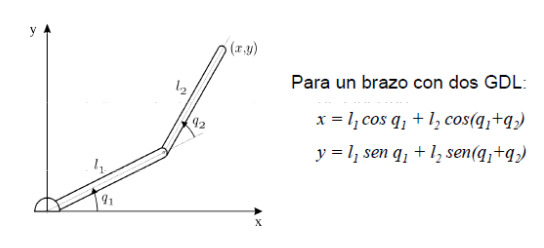
\includegraphics[width=8cm]{4.jpg}
\caption{Cinem\'atica Inversa}
\label{Figura 4}
\end{figure}

La primera variables articular se calcula de la sigueinte manera:

\begin{displaymath}
\theta_1 = atan2(x_c, y_c)
\end{displaymath}

Siempre y cuando $x_c, y_c$ ambas no sean cero.

De la figura 4, el \'angulo $\theta_2$ se calcula de la siguente manera:

\begin{displaymath}
\theta_2 =atan2(r,s)+ \frac{n}{2}
\end{displaymath}

Donde:

\begin{displaymath}
r^2=x^2_c+y^2_c,s=z_c-d_1
\end{displaymath}

La distancia lineal $d_3$ se calcula como sigue:

\begin{displaymath}
d_3=\sqrt{r^2+s^2}=\sqrt{x^2_c+y^2_c+(z^2_c-d_1)}
\end{displaymath}

En cuanto a la cinem\'atica inversa de orientaci\'on, las \'ultimas dos variables articulares $\theta_4$, $\theta_5$ se calculan utilizando los \'angulos de Euler. Dada una matriz R denotando la orientaci\'on deseada del marco del efector final respecto del marco inercia y la amtriz de rotaci\'on $R^3_0$ es posible encontrar $\theta_4$ y $\theta_5$, como a continuaci\'on se muestra.

 Matriz $R^3_0$

\begin{center}
$R^3_0$=[$\begin{matrix}
	cos\theta_1cos\theta_2 & -cos\theta_1sin\theta_2 & -sin\theta_1 & -(cos\theta_1sin\theta_2)d_3\\
	sin\theta_1cos\theta_2 & -sin\theta_1sin\theta_2 & cos\theta_1 & -(sin\theta_1sin\theta_2)d_3\\
	-sin\theta_2 & -cos\theta_2 & 0 & -(cos\theta_2)d_3+d_1\\
	0 & 0 & 0 & 1
\end{matrix}$ ]
\end{center}

Matriz $R^5_3$

\begin{center}
$R^5_3$=[$\begin{matrix}
	cos\theta_4cos\theta_5 & -cos\theta_4sin\theta_5 & -sin\theta_4\\
	sin\theta_4cos\theta_5 & -sin\theta_4sin\theta_5 & cos\theta_4\\
	-sin\theta_5 & cos\theta_5 & 0 \\
\end{matrix}$ ]
\end{center}

Y la soluci\'on de Euler se puede aplicar en la siguiente ecuaci\'on:

\begin{displaymath}
R^5_3=(R^3_0)^TR
\end{displaymath}

\begin{displaymath}
-S_4=C_12r_13+S_1C_2r_23-S_2r_33
\end{displaymath}

\begin{displaymath}
C_4=-C_1S_2r_13-S_12r_23-C_2r_33
\end{displaymath}

\begin{displaymath}
\theta_4=atan2(-S_4)
\end{displaymath}

\begin{displaymath}
\theta_5=atan2(C_4)
\end{displaymath}
\section{Referencias}
@article{de2017ingenieria,
  title={INGENIER{\'I}A MECATR{\'O}NICA EN COMPETENCIAS PROFESIONALES},
  author={DE ROBOTS, ASIGNATURA DE CINEMATICA},
  year={2017}
}
@mastersthesis{granja2014modelacion,
  title={Modelaci{\'o}n y an{\'a}lisis de la cinem{\'a}tica directa e inversa del manipulador Stanford de seis grados de libertad},
  author={Granja Oramas, Mar{\'\i}a Victoria},
  type={{B.S.} thesis},
  year={2014},
  school={Quito, 2014.}
}
\bibliographystyle{apalike}
\bibliography{biblio}
\end{document}
